This section shows kinematic distributions of events in the range of 
$120<\mt<140~\GeV$ and $25<\mll<50~\GeV$ for 2D analysis in DF 0/1jet bins.   
All backgrounds are normalized to the estimation.

%MET 
\begin{figure}[!hbtp]
\centering
\subfigure[]{
\centering
\label{subfig:hww125_pmet_0j}
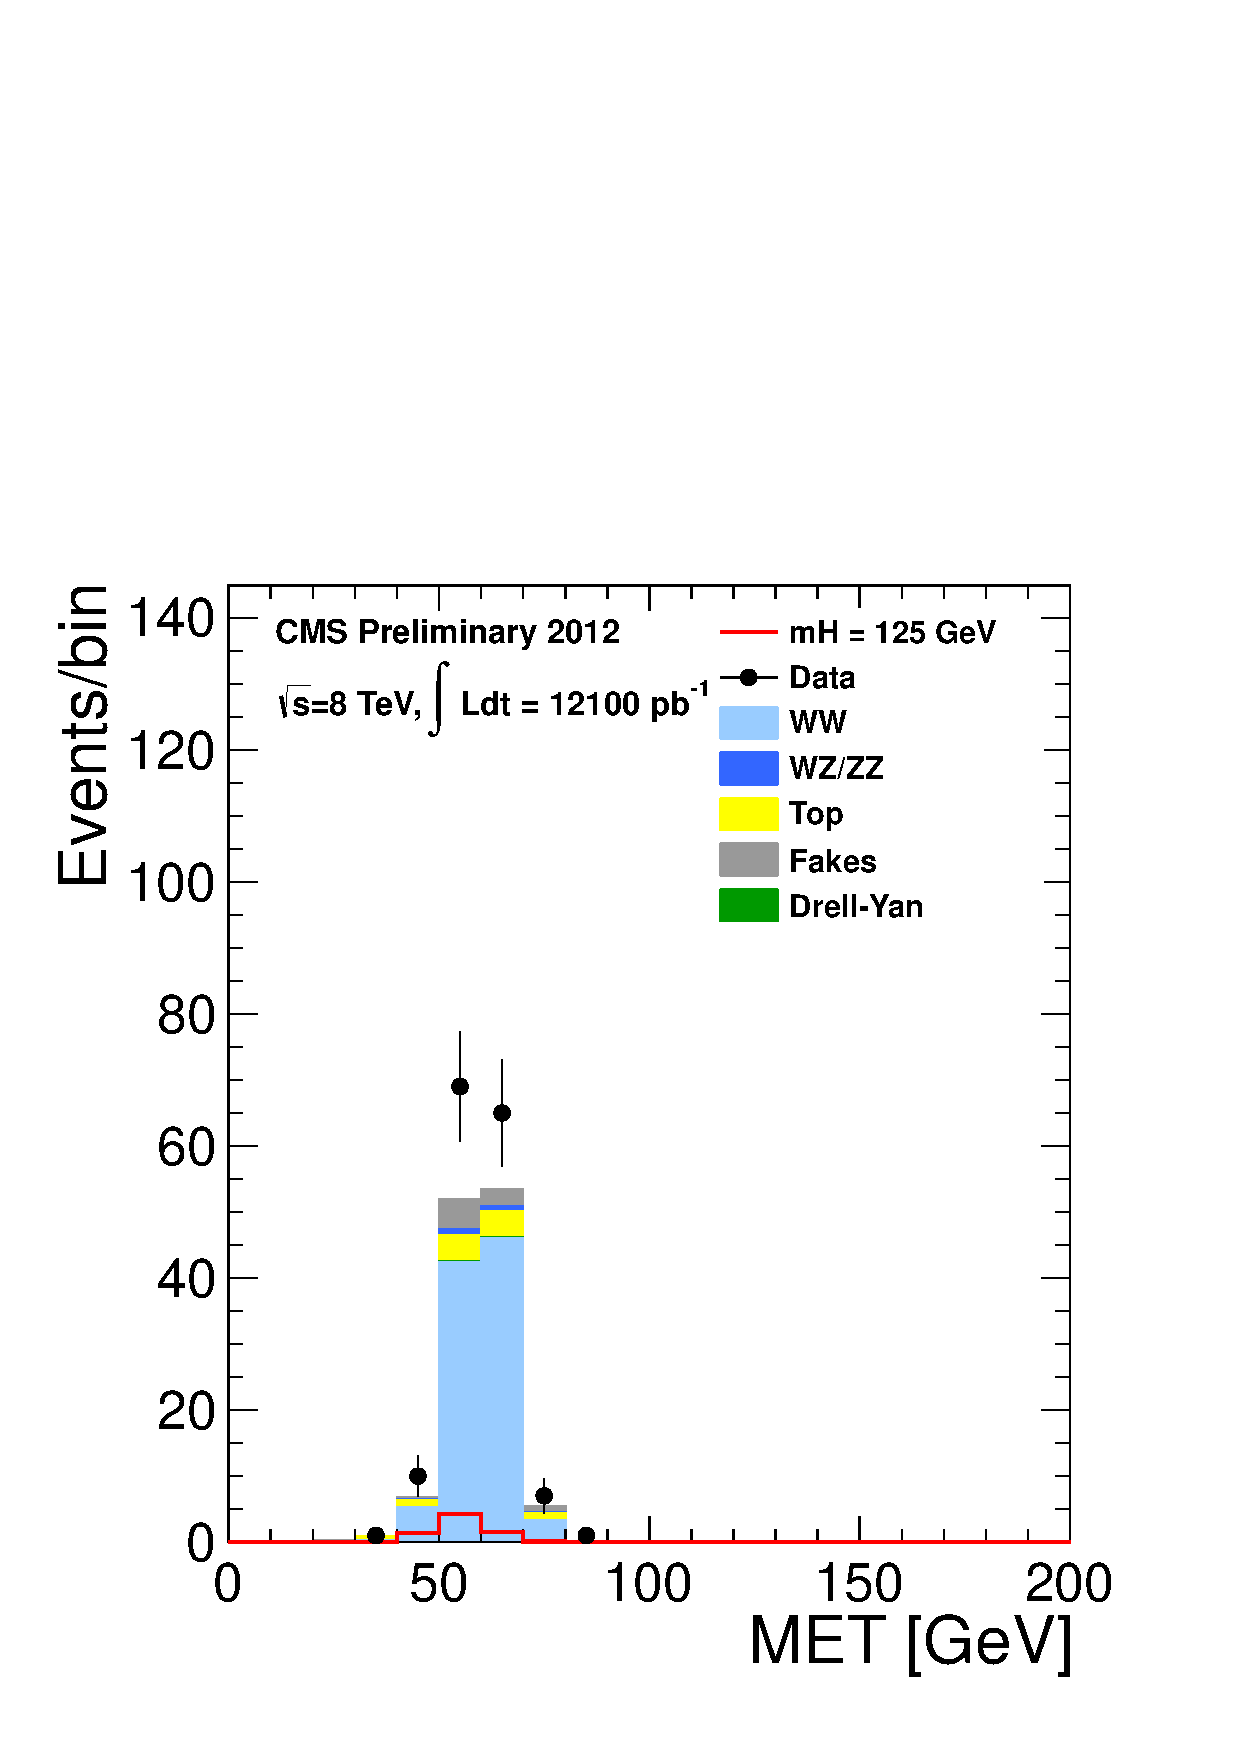
\includegraphics[width=.3\textwidth]{figures/hwwplots_mt120to140_mll25to50/hww_analysis18_125_ALL_of_0j_met.pdf}
}
\subfigure[]{
\centering
\label{subfig:hww125_pmet_1j}
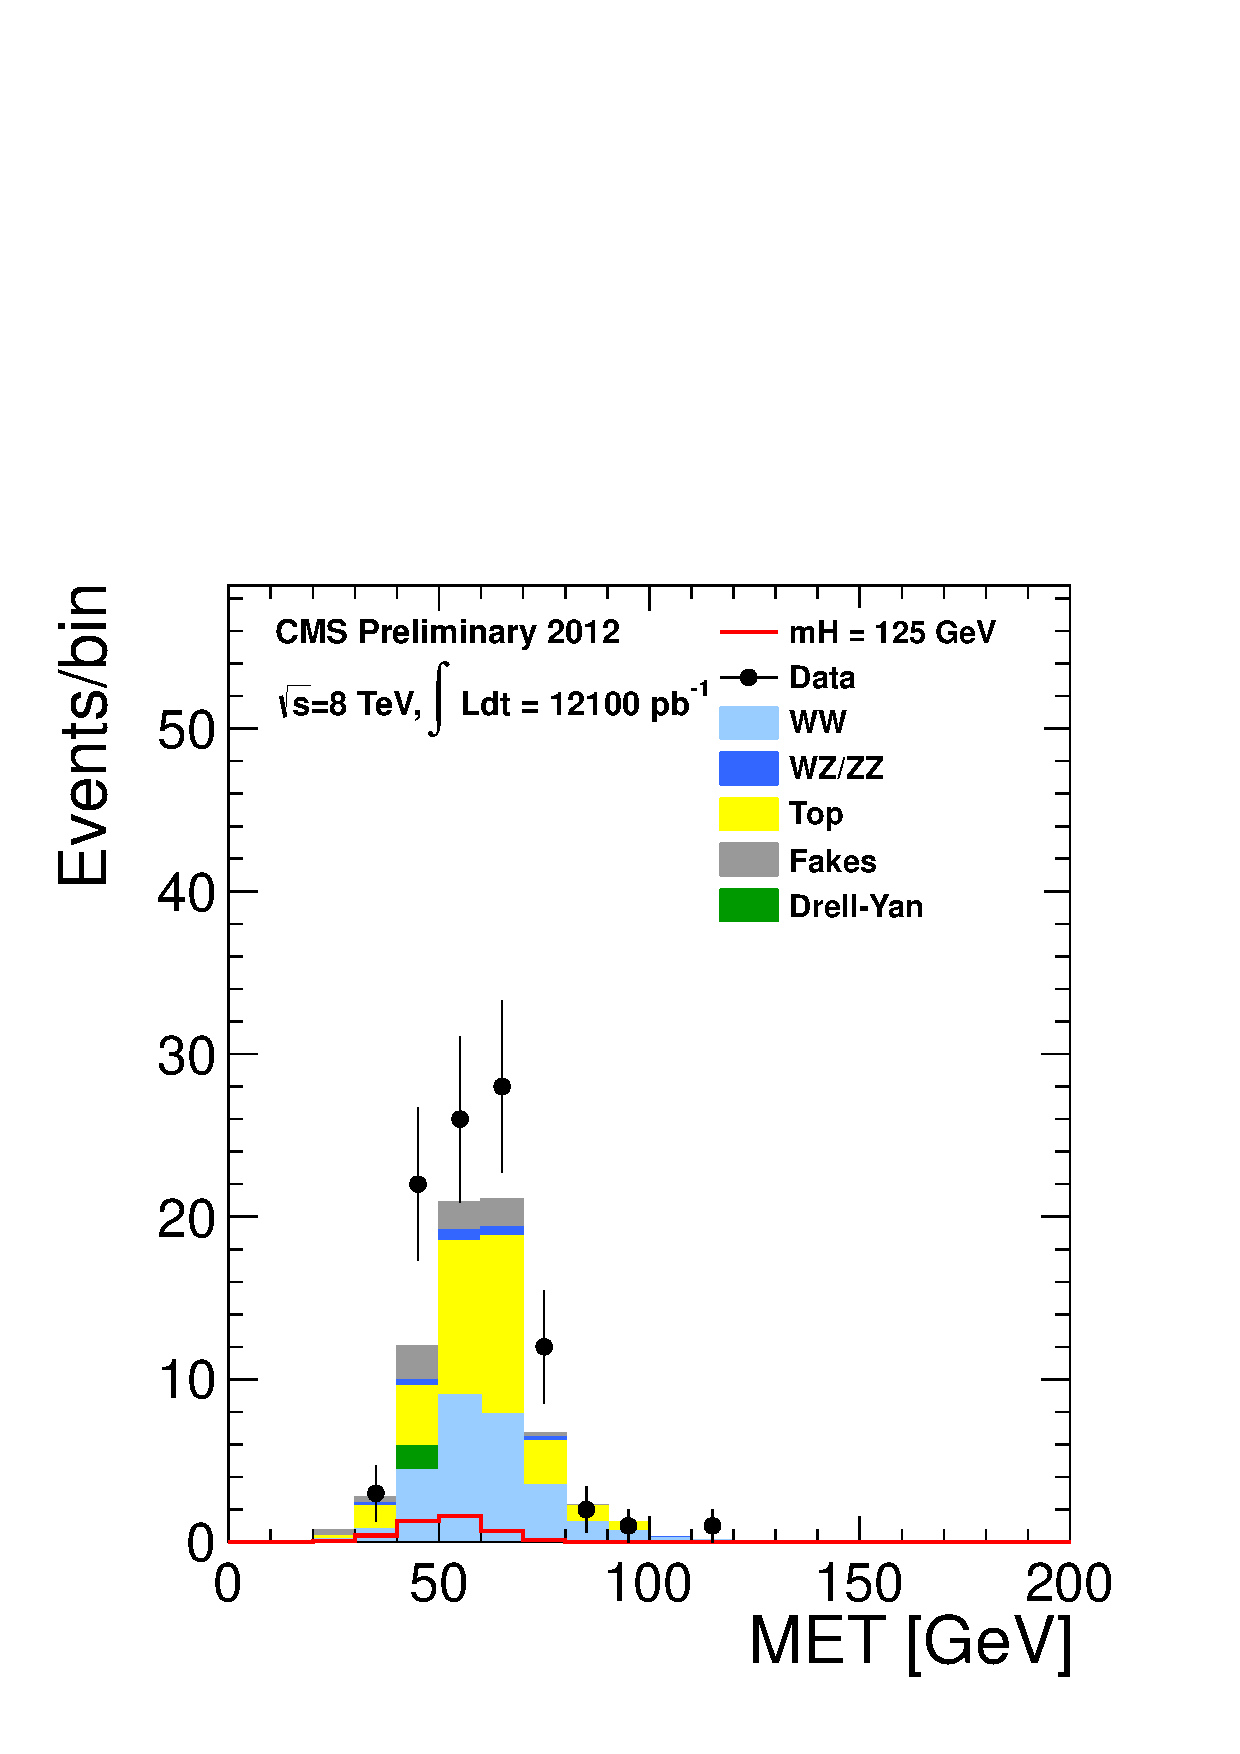
\includegraphics[width=.3\textwidth]{figures/hwwplots_mt120to140_mll25to50/hww_analysis18_125_ALL_of_1j_met.pdf}
}
\caption{The $\met$ distributions for $\mHi=125~\GeV$ with \intlumiEightTeV~of data in the 0-jet \subref{subfig:hww125_pmet_0j},
1-jet \subref{subfig:hww125_pmet_1j} bin analyses.}
\label{fig:hww125_pmet}
\end{figure} 


%dPhi 
\begin{figure}[!hbtp]
\centering
\subfigure[]{
\centering
\label{subfig:hww125_dphi_0j}
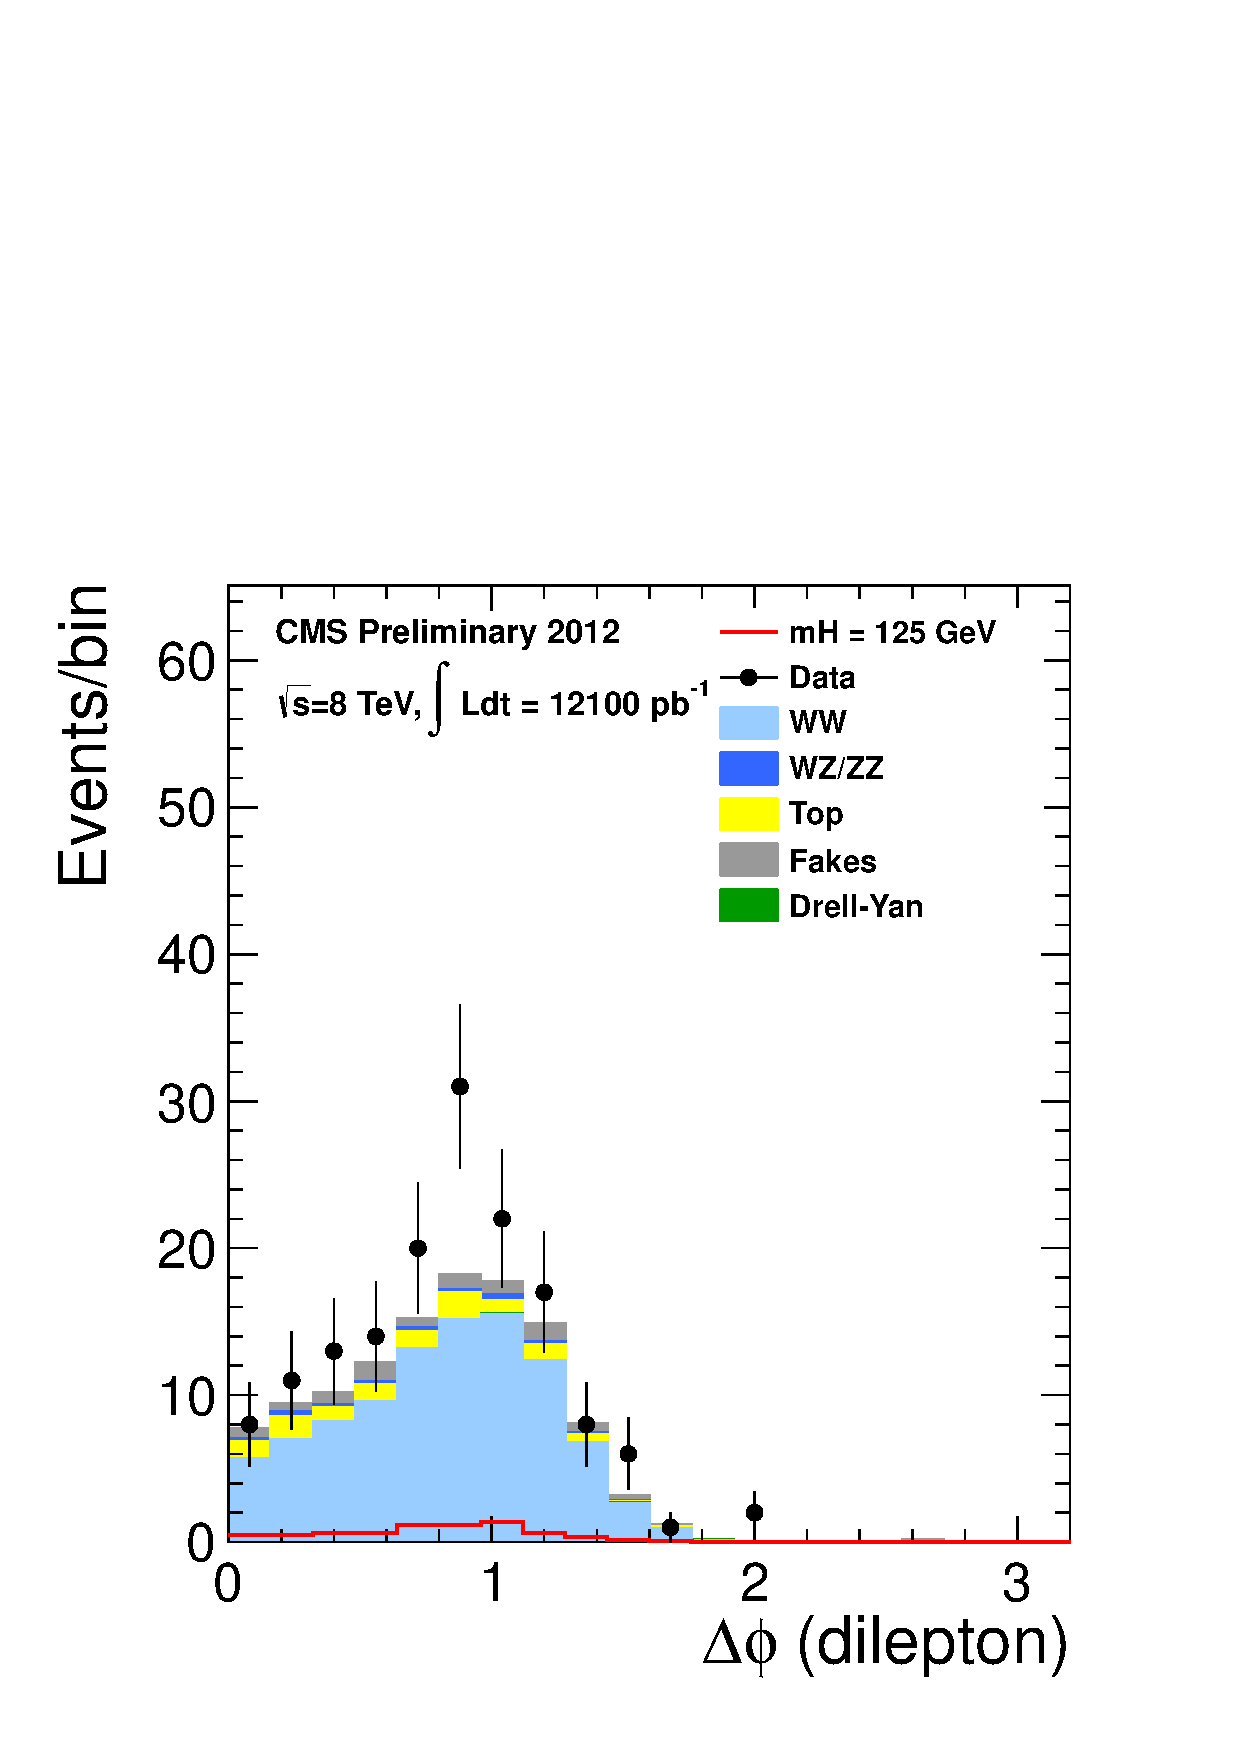
\includegraphics[width=.3\textwidth]{figures/hwwplots_mt120to140_mll25to50/hww_analysis18_125_ALL_of_0j_dphi.pdf}
}
\subfigure[]{
\centering
\label{subfig:hww125_dphi_1j}
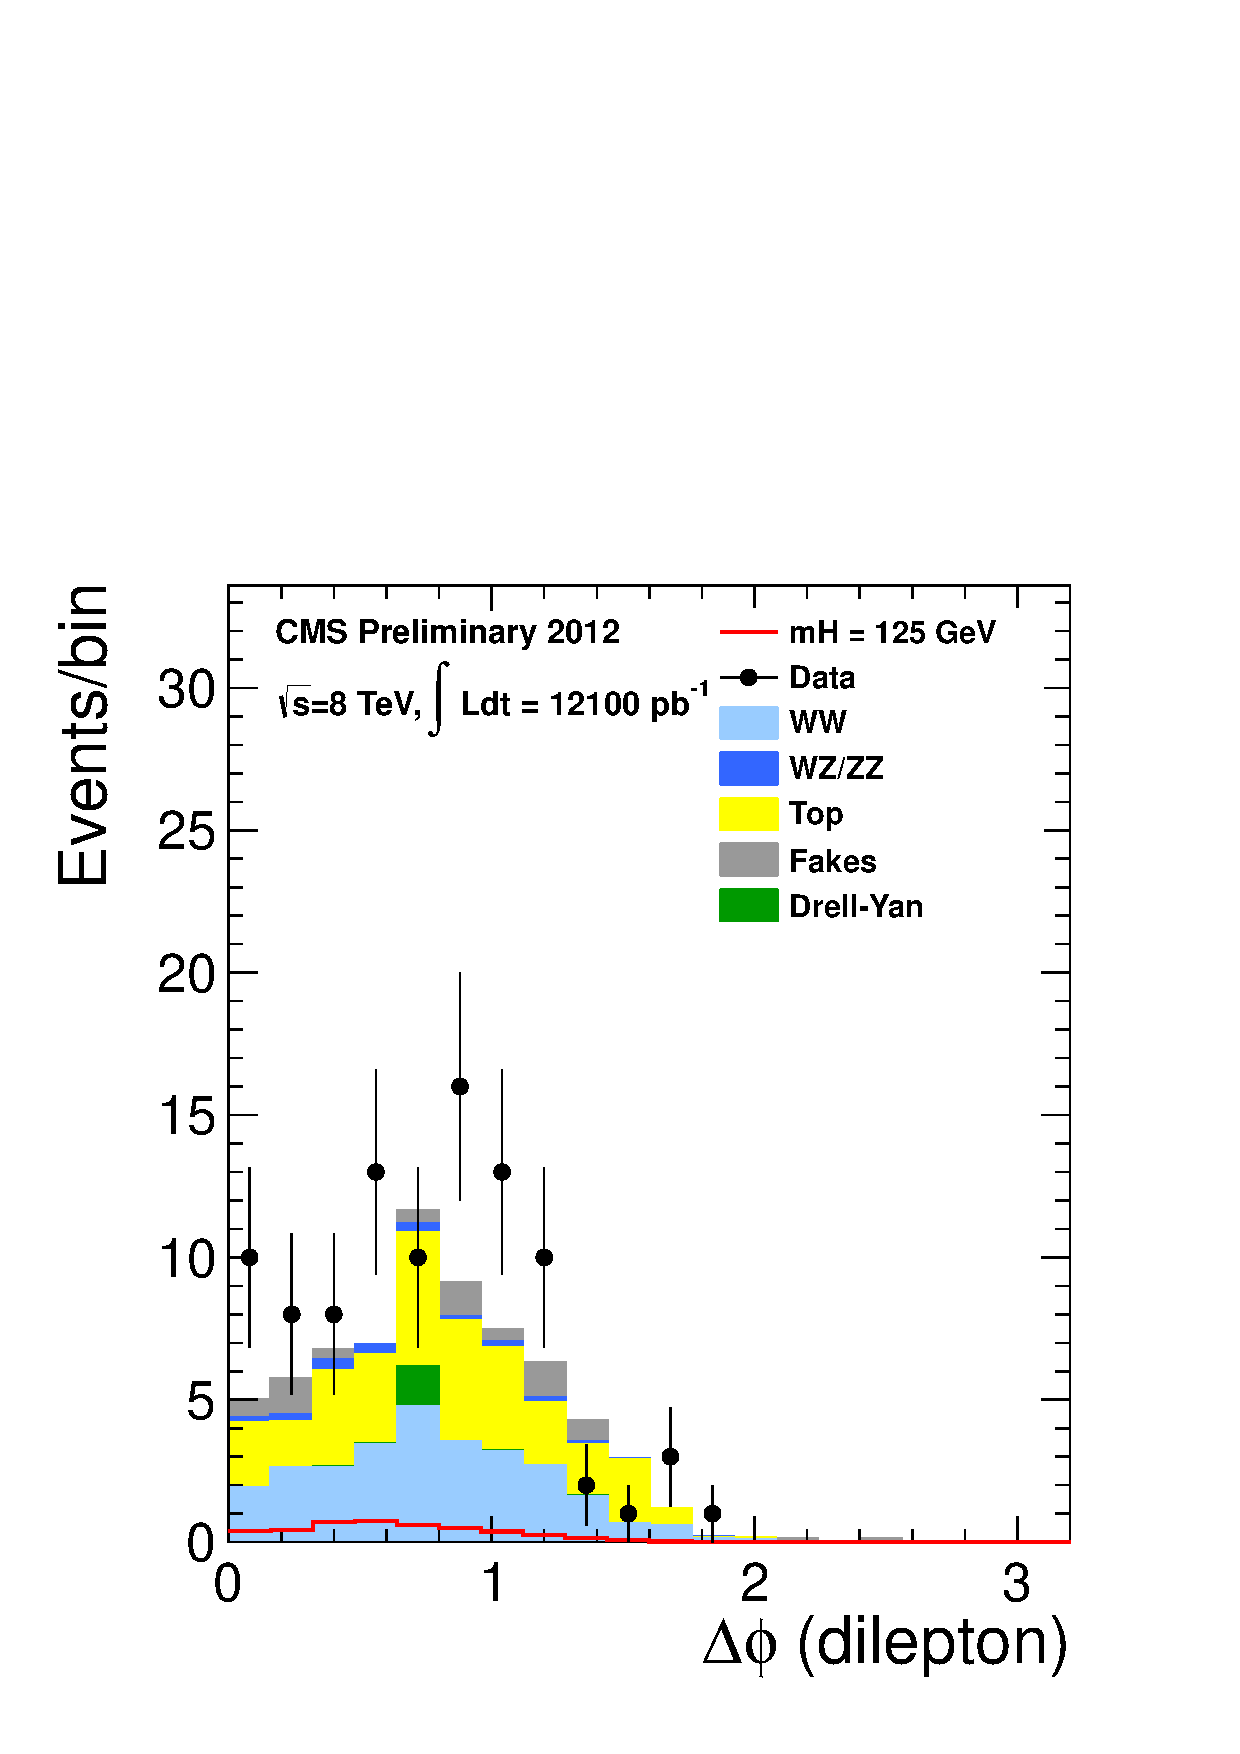
\includegraphics[width=.3\textwidth]{figures/hwwplots_mt120to140_mll25to50/hww_analysis18_125_ALL_of_1j_dphi.pdf}
}
\caption{The \delphill distributions for $\mHi=125~\GeV$ with \intlumiEightTeV~of data in the 0-jet \subref{subfig:hww125_dphi_0j},
1-jet \subref{subfig:hww125_dphi_1j} bin analyses.}
\label{fig:hww125_dphi}
\end{figure} 

%mll 
\begin{figure}[!hbtp]
\centering
\subfigure[]{
\centering
\label{subfig:hww125_mll_0j}
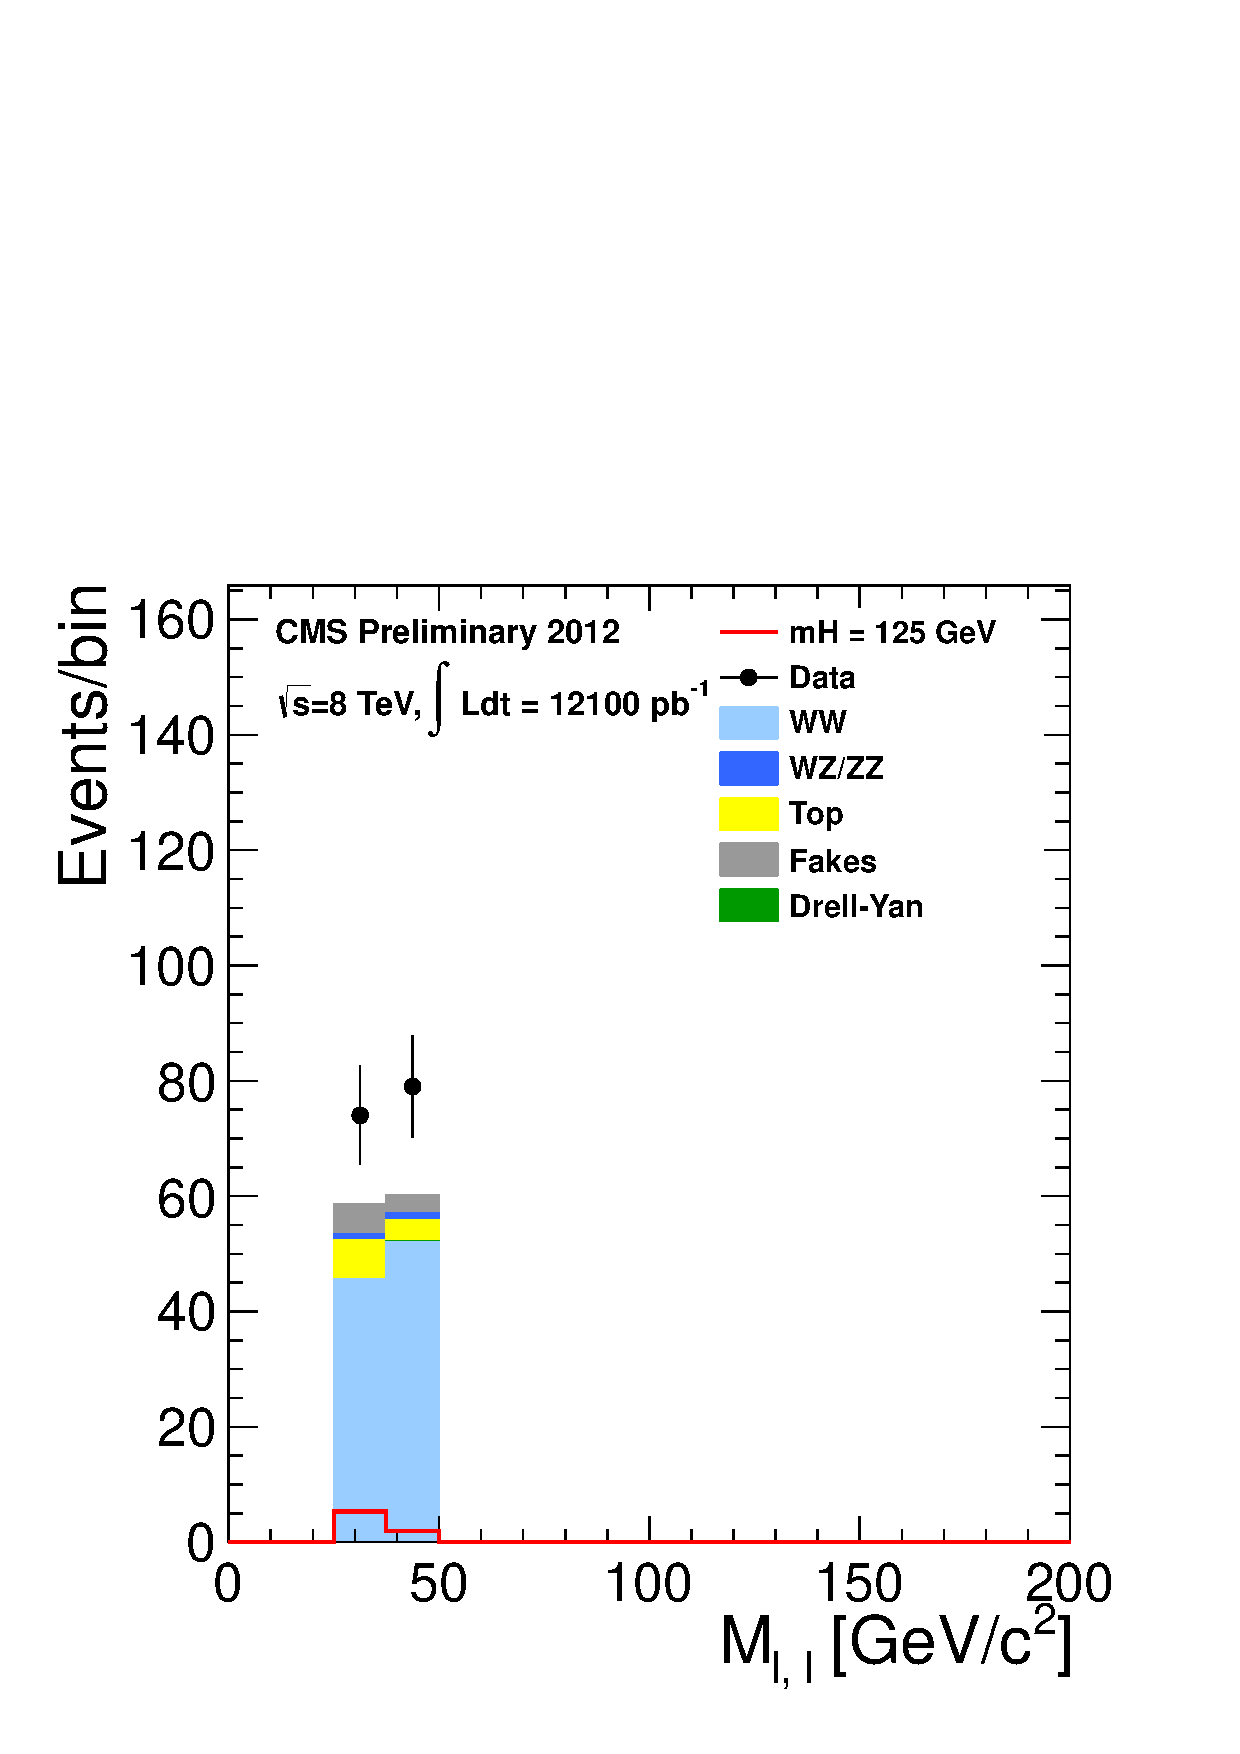
\includegraphics[width=.3\textwidth]{figures/hwwplots_mt120to140_mll25to50/hww_analysis18_125_ALL_of_0j_mll.pdf}
}
\subfigure[]{
\centering
\label{subfig:hww125_mll_1j}
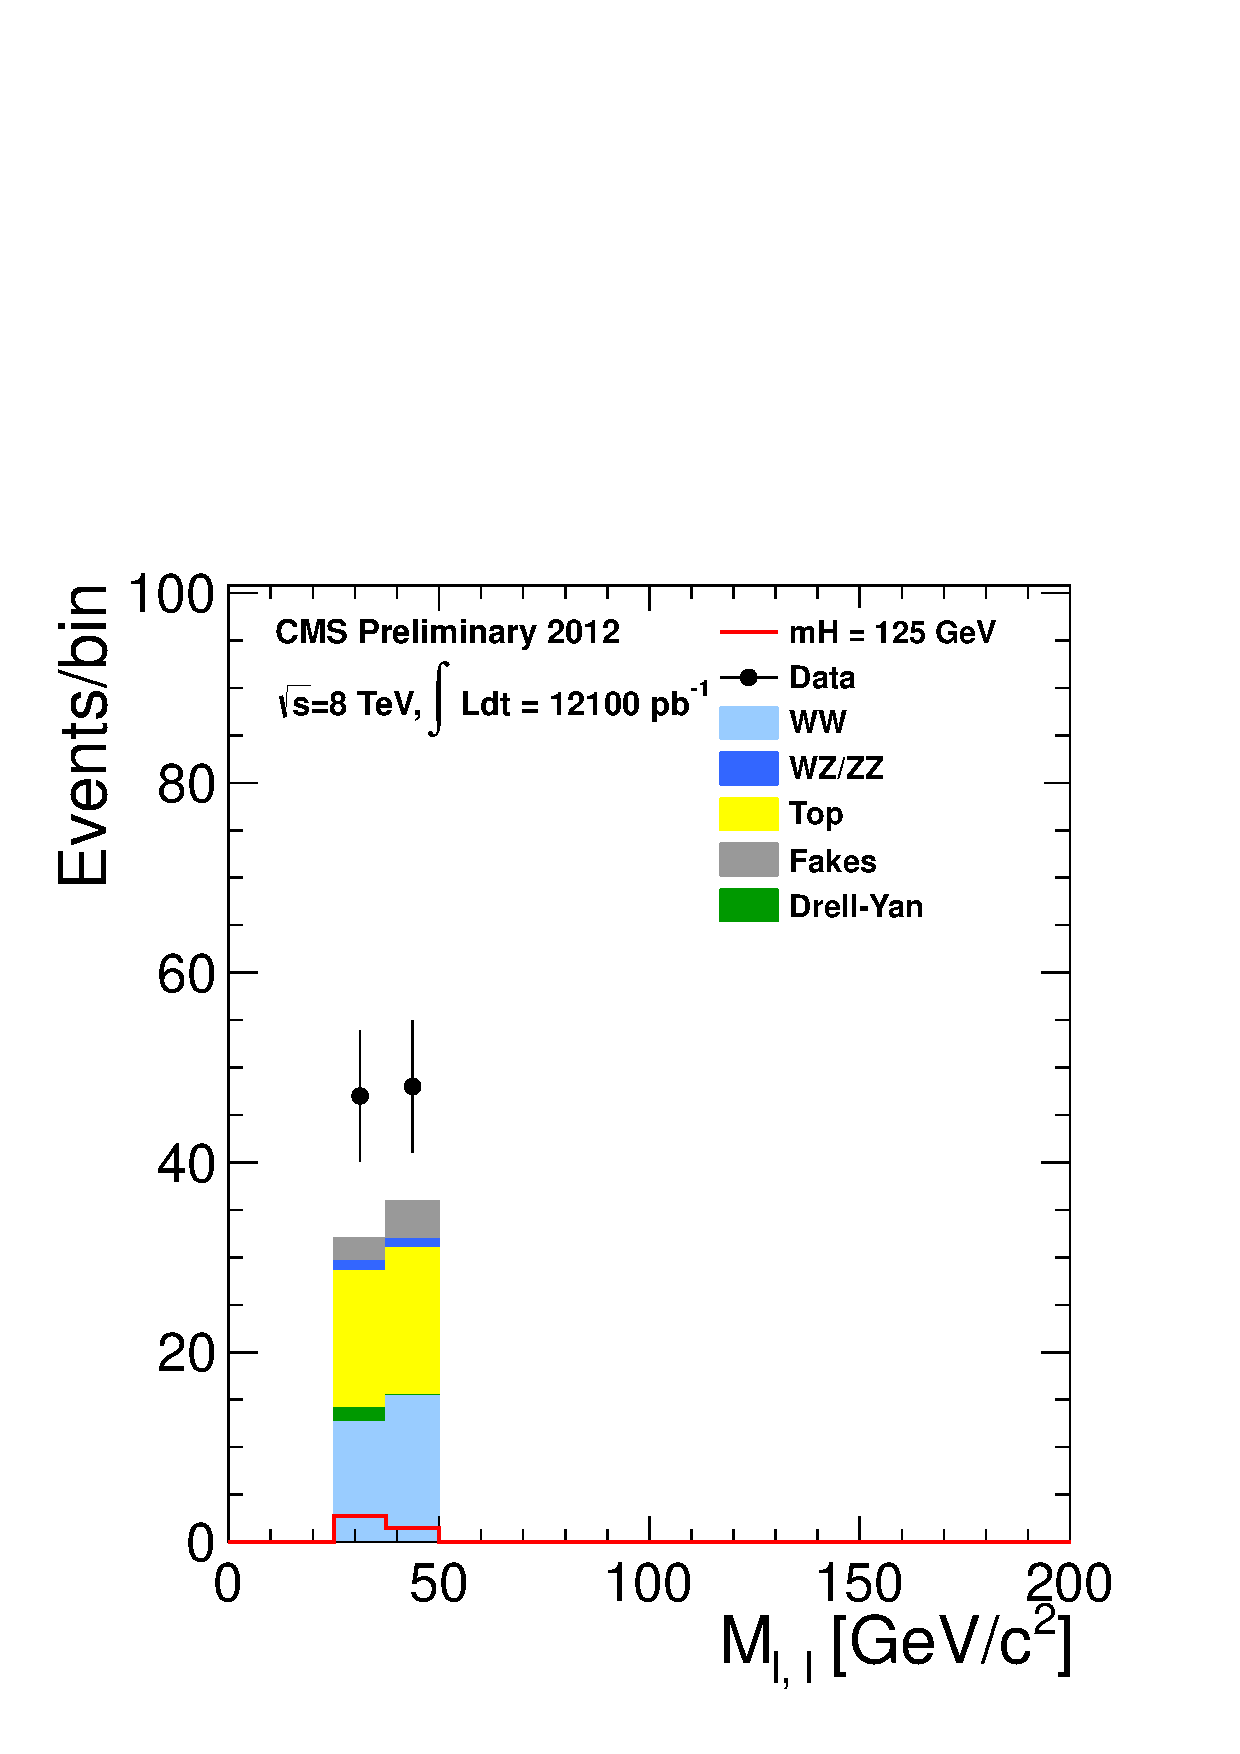
\includegraphics[width=.3\textwidth]{figures/hwwplots_mt120to140_mll25to50/hww_analysis18_125_ALL_of_1j_mll.pdf}
}
\caption{The \mll~distributions for $\mHi=125~\GeV$ with \intlumiEightTeV~ of data in the 0-jet \subref{subfig:hww125_mll_0j},
1-jet \subref{subfig:hww125_mll_1j} bin analyses.}
\label{fig:hww125_mll}
\end{figure} 

%mT 
\begin{figure}[!hbtp]
\centering
\subfigure[]{
\centering
\label{subfig:hww125_mt_0j}
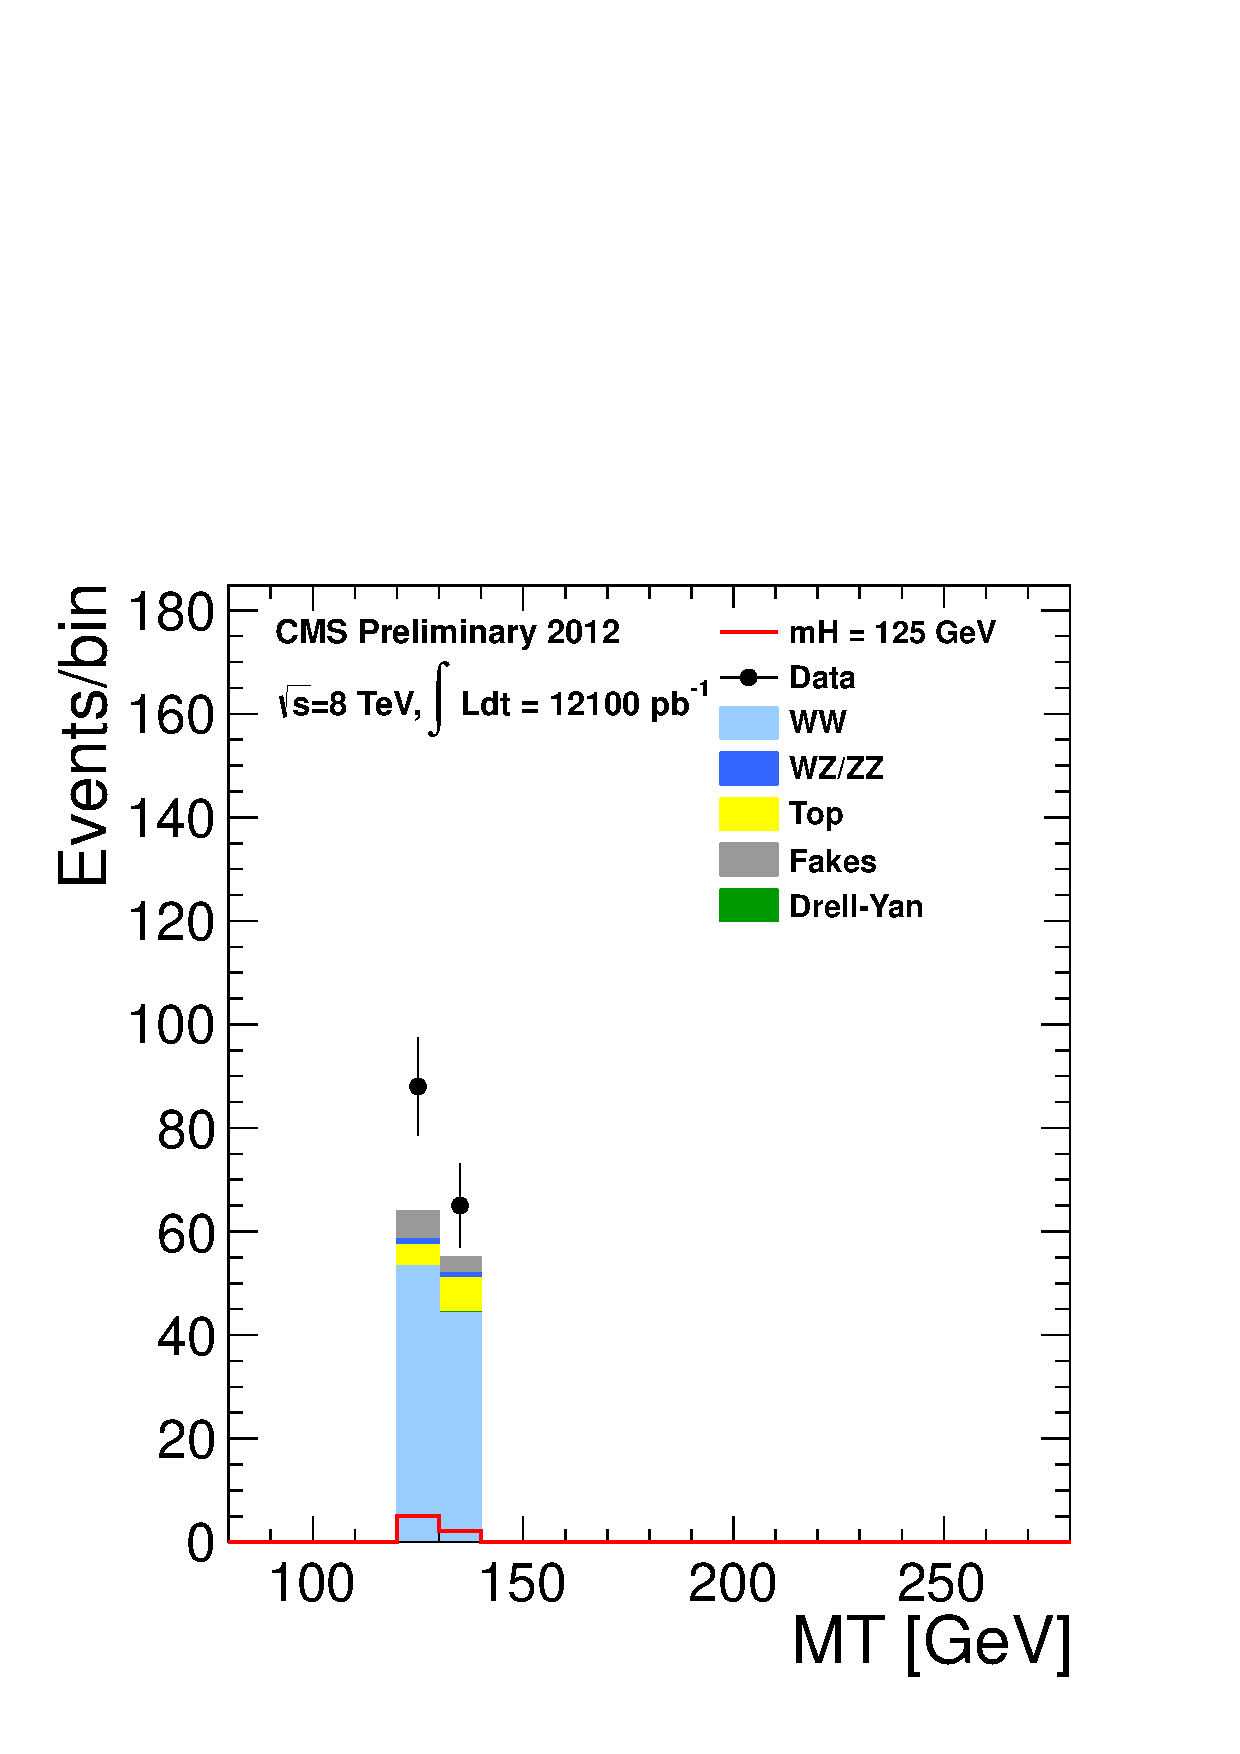
\includegraphics[width=.3\textwidth]{figures/hwwplots_mt120to140_mll25to50/hww_analysis18_125_ALL_of_0j_mt.pdf}
}
\subfigure[]{
\centering
\label{subfig:hww125_mt_1j}
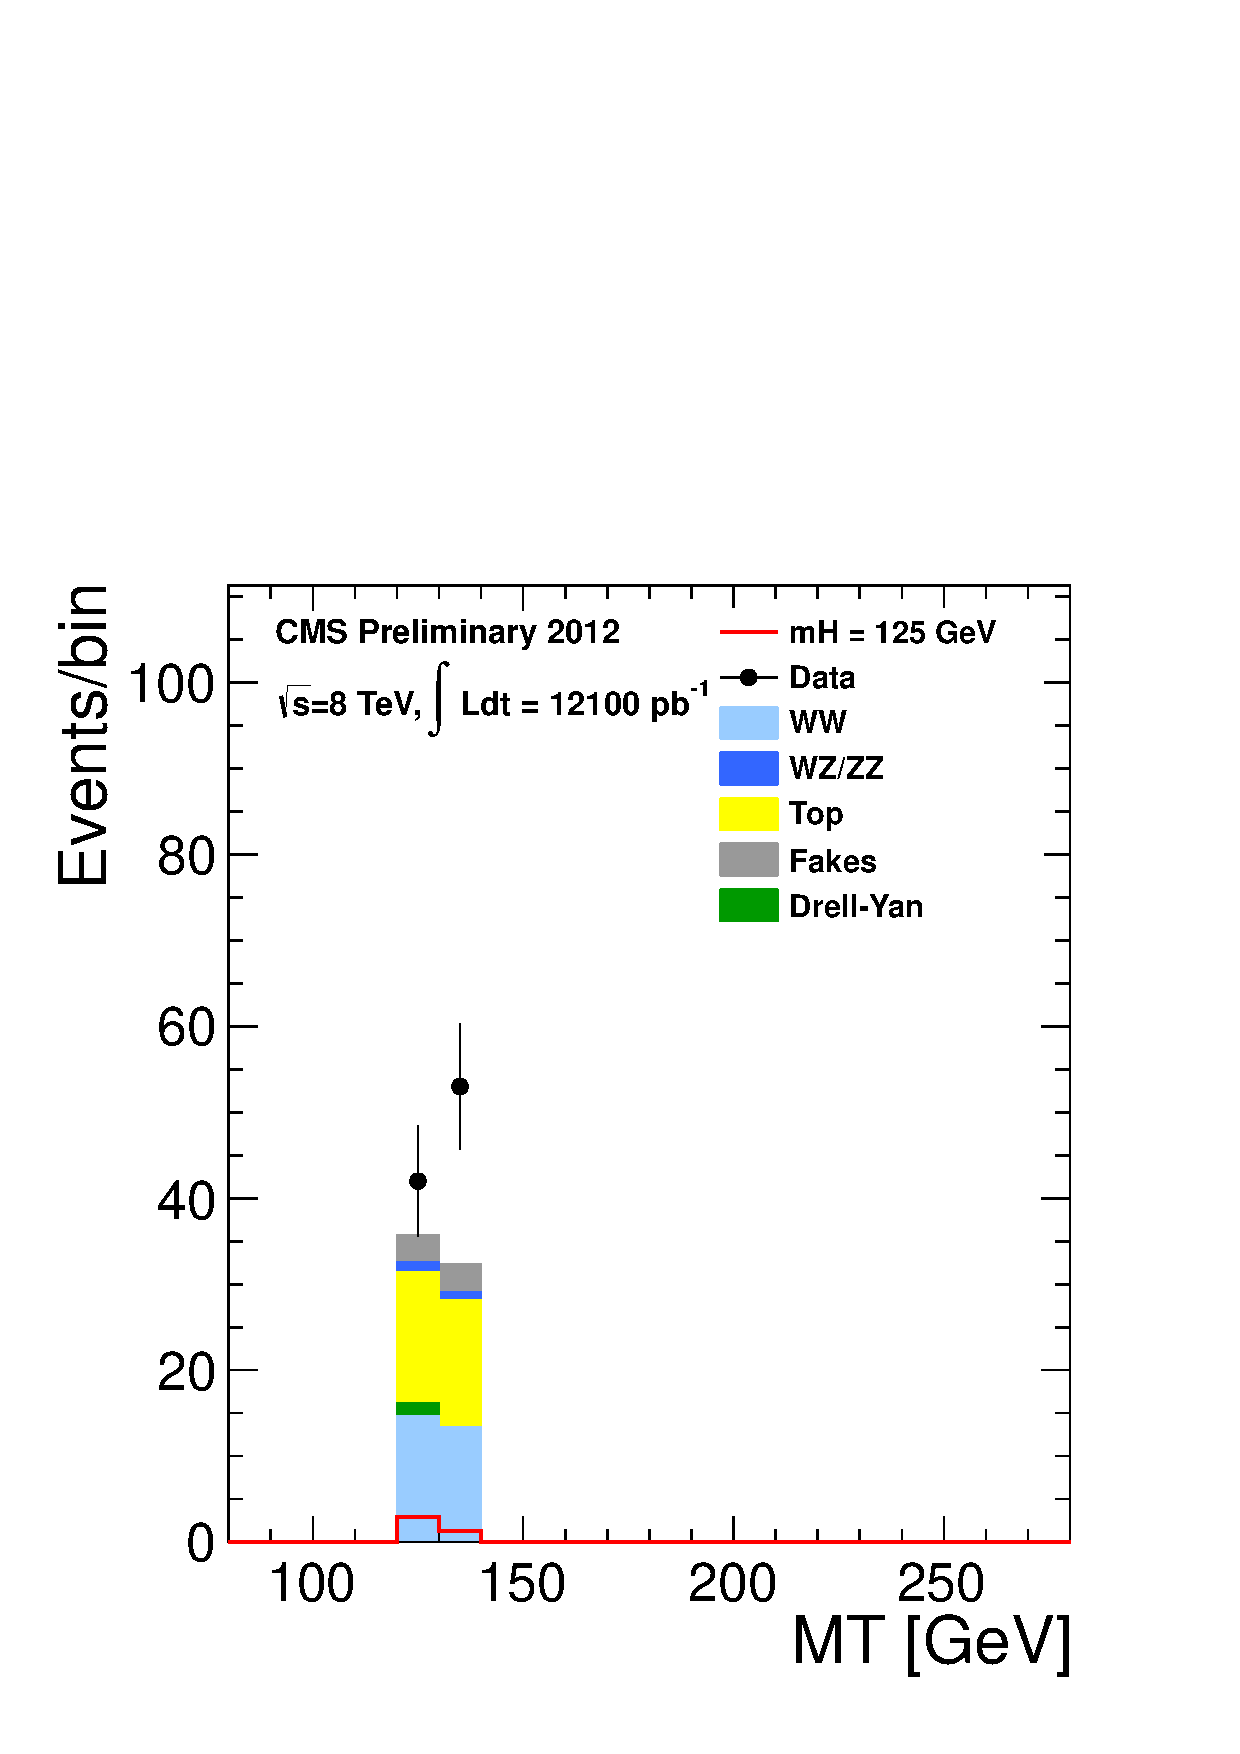
\includegraphics[width=.3\textwidth]{figures/hwwplots_mt120to140_mll25to50/hww_analysis18_125_ALL_of_1j_mt.pdf}
}
\caption{The \mt~distributions for $\mHi=125~\GeV$ with \intlumiEightTeV~of data in the 0-jet \subref{subfig:hww125_mt_0j},
1-jet \subref{subfig:hww125_mt_1j} bin analyses.}
\label{fig:hww125_mt}
\end{figure} 

%pT1 
\begin{figure}[!hbtp]
\centering
\subfigure[]{
\centering
\label{subfig:hww125_pt1_0j}
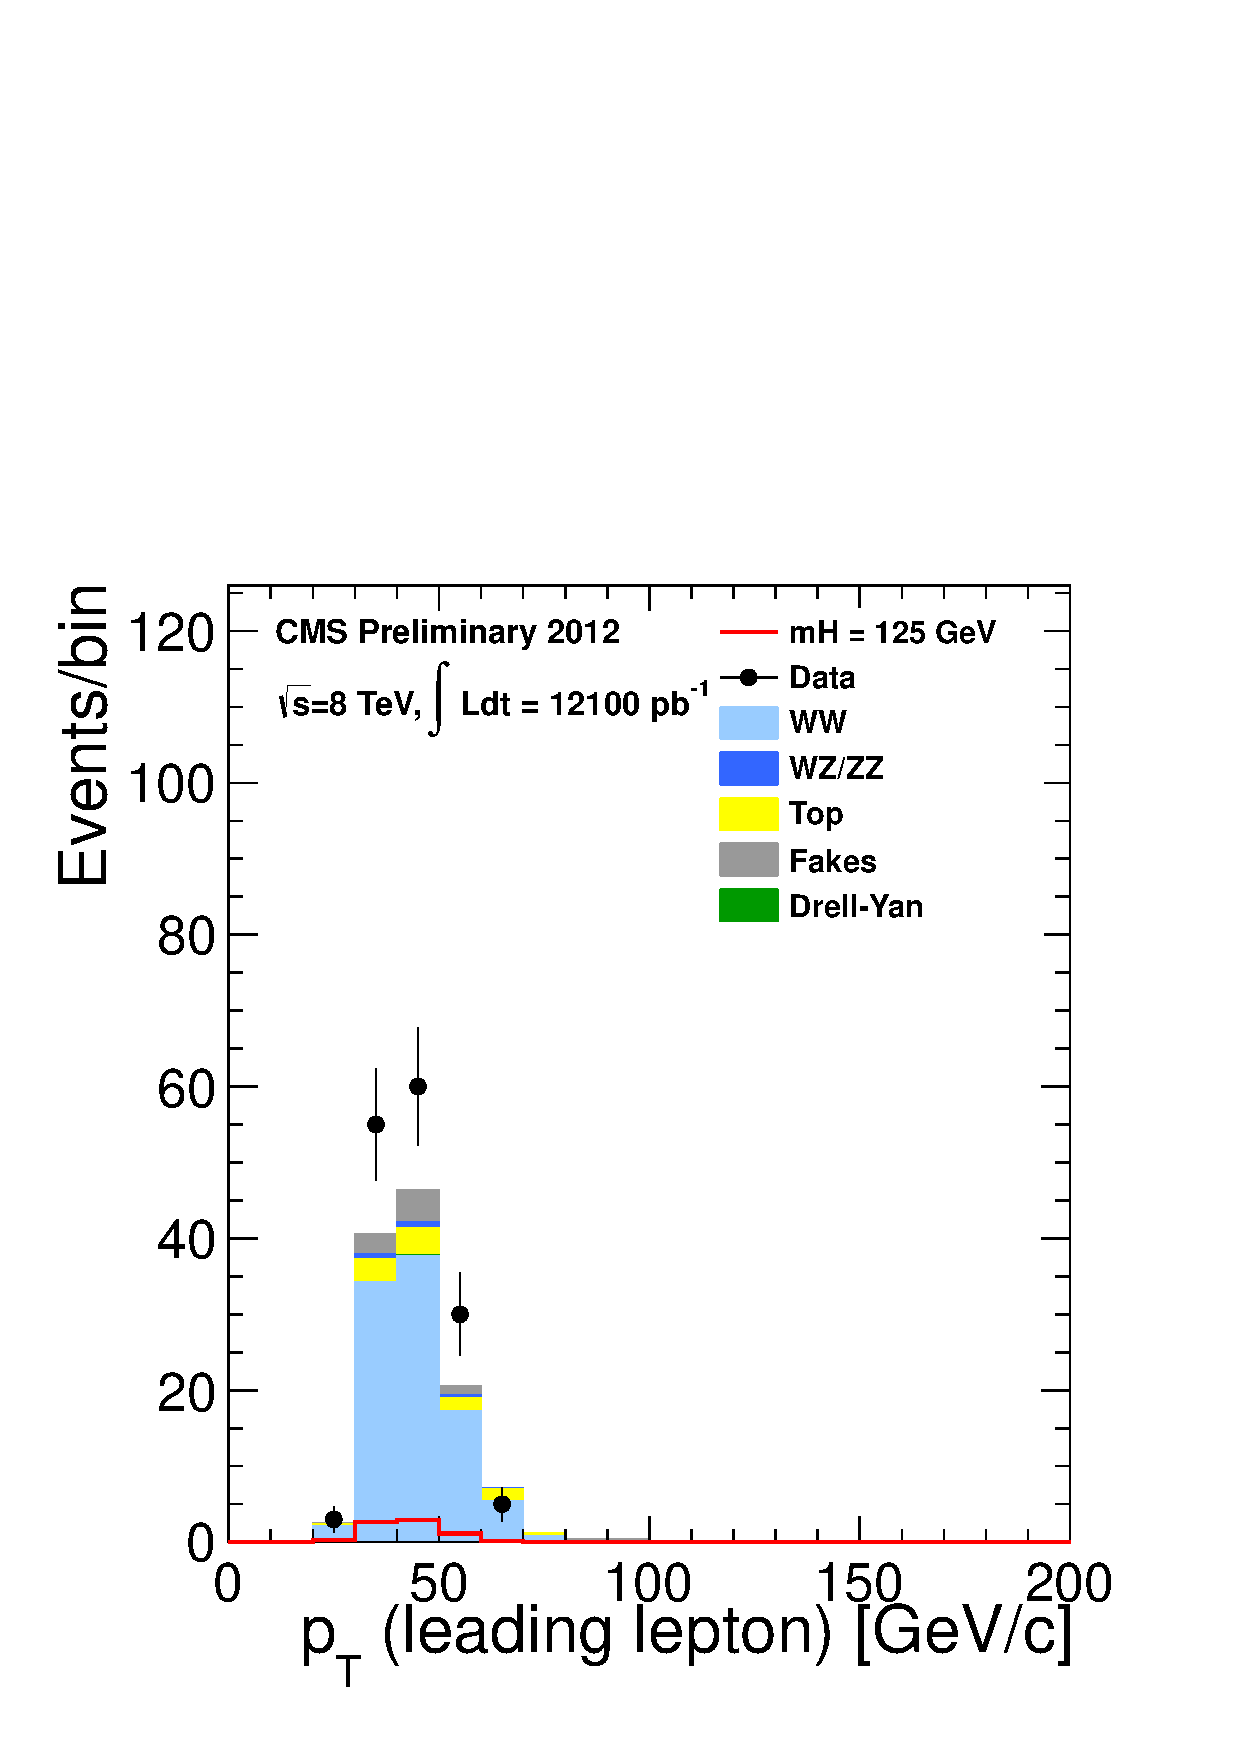
\includegraphics[width=.3\textwidth]{figures/hwwplots_mt120to140_mll25to50/hww_analysis18_125_ALL_of_0j_pt1.pdf}
}
\subfigure[]{
\centering
\label{subfig:hww125_pt1_1j}
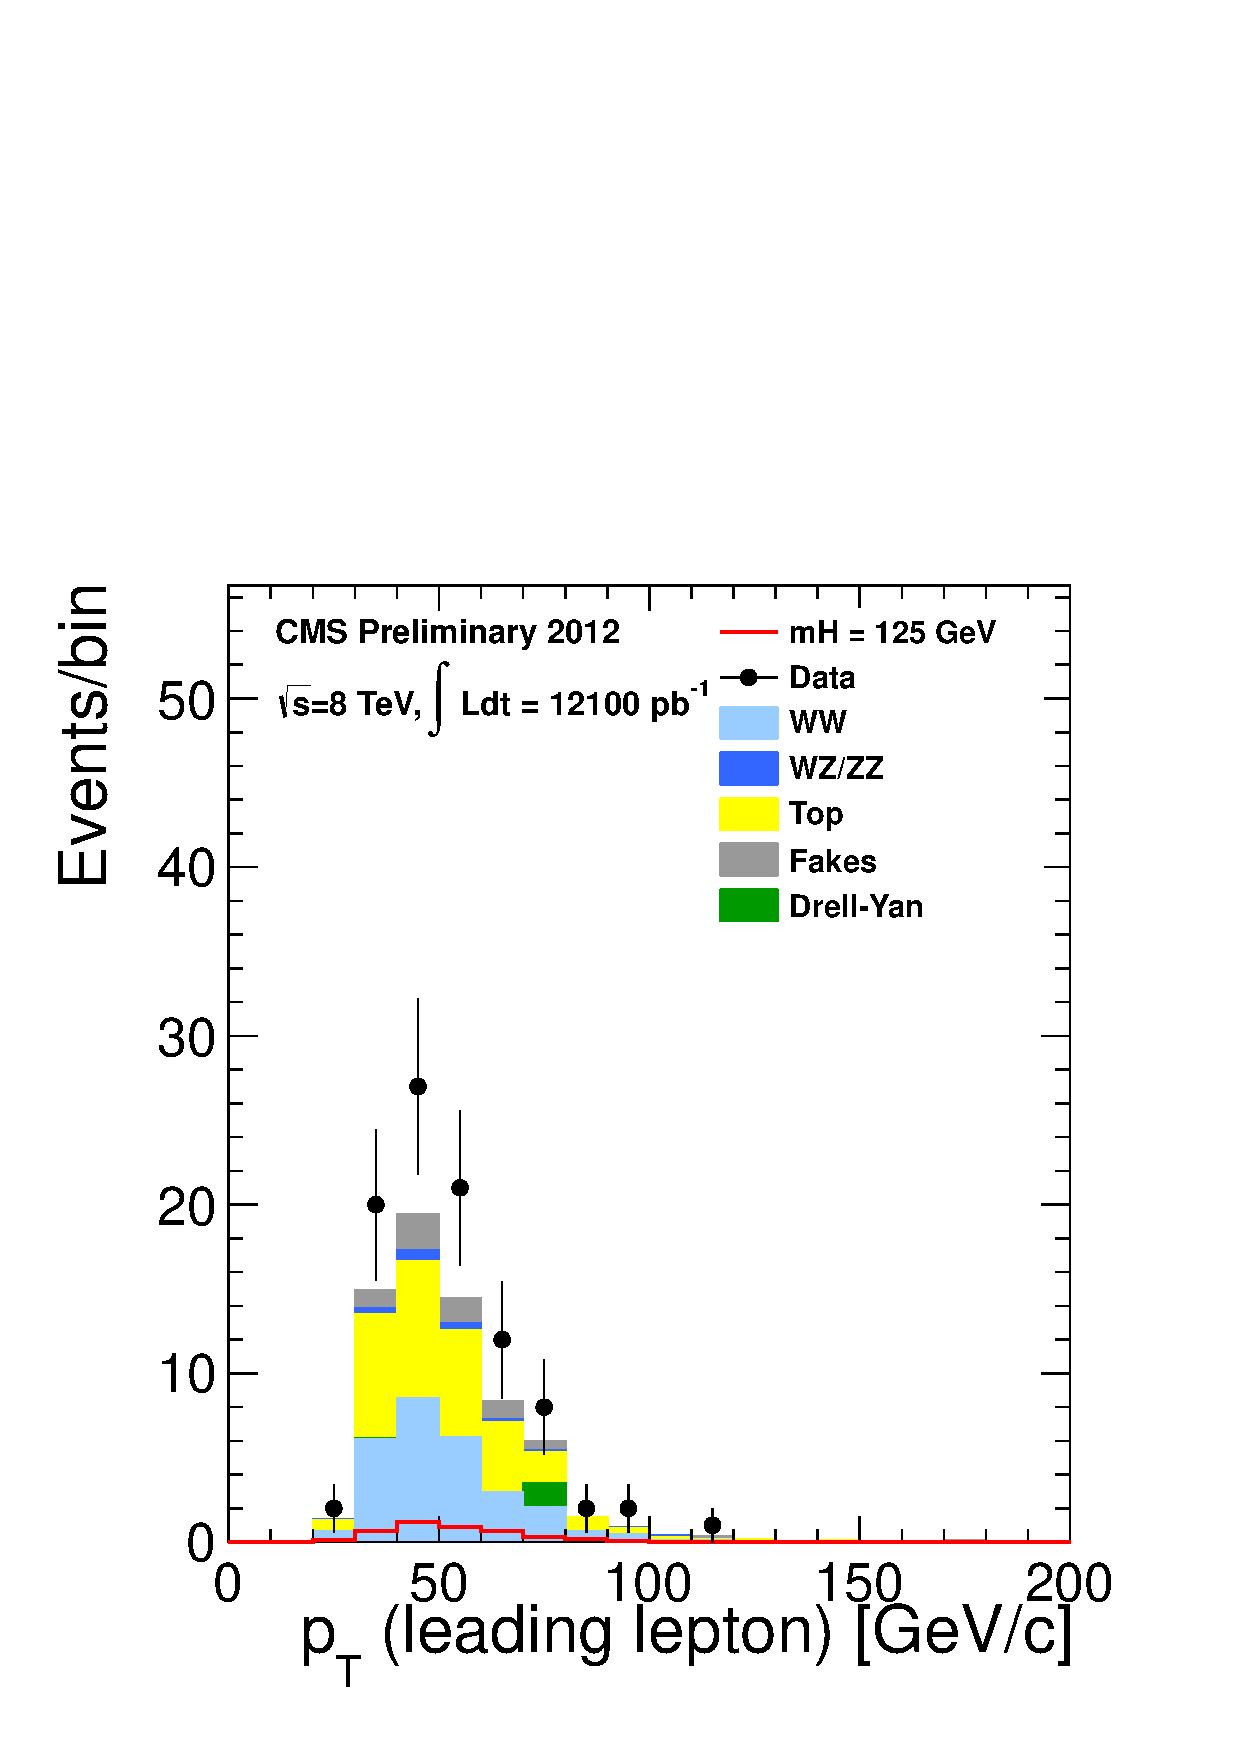
\includegraphics[width=.3\textwidth]{figures/hwwplots_mt120to140_mll25to50/hww_analysis18_125_ALL_of_1j_pt1.pdf}
}
\caption{The \ptlmax~distributions for $\mHi=125~\GeV$ with \intlumiEightTeV~of data in the 0-jet \subref{subfig:hww125_pt1_0j},
1-jet \subref{subfig:hww125_pt1_1j} bin analyses.}
\label{fig:hww125_pt1}
\end{figure} 

%pT2
\begin{figure}[!hbtp]
\centering
\subfigure[]{
\centering
\label{subfig:hww125_pt2_0j}
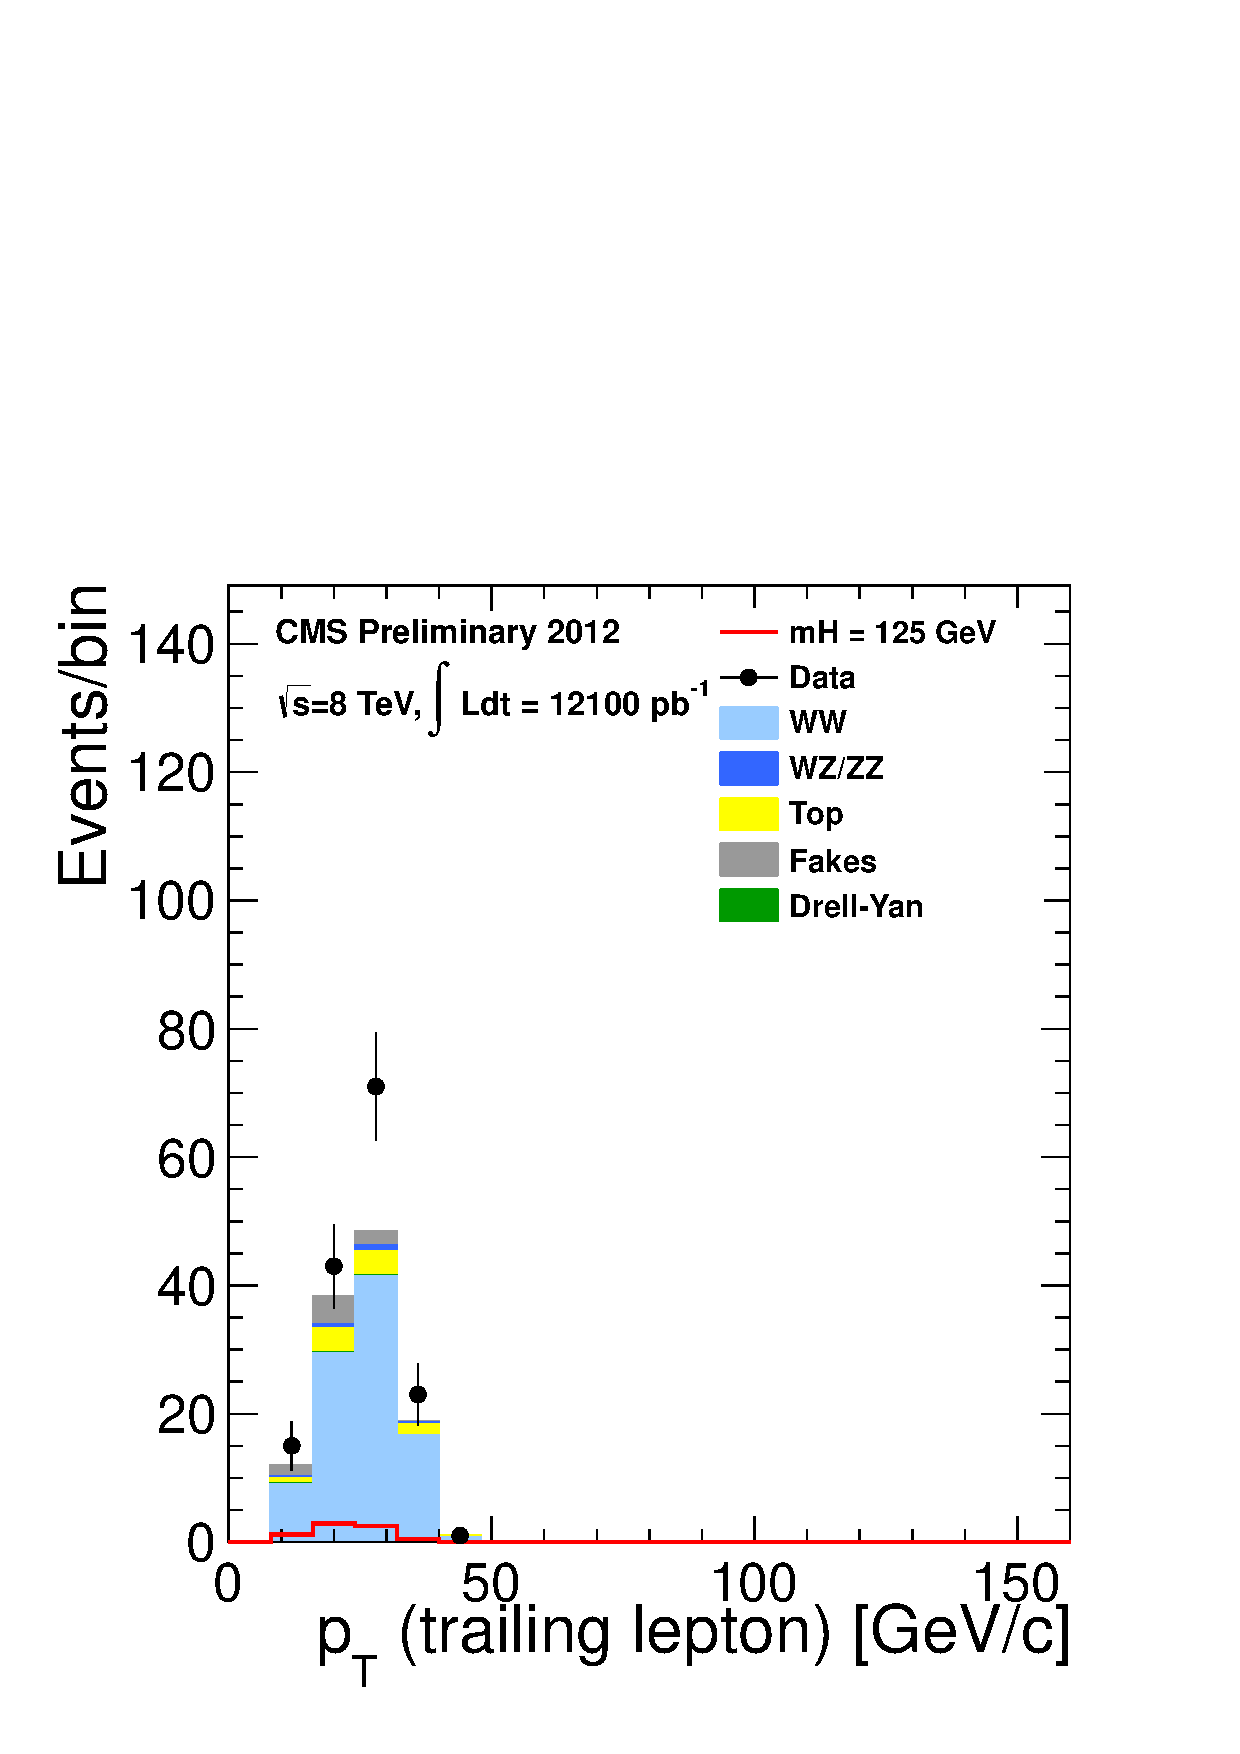
\includegraphics[width=.3\textwidth]{figures/hwwplots_mt120to140_mll25to50/hww_analysis18_125_ALL_of_0j_pt2.pdf}
}
\subfigure[]{
\centering
\label{subfig:hww125_pt2_1j}
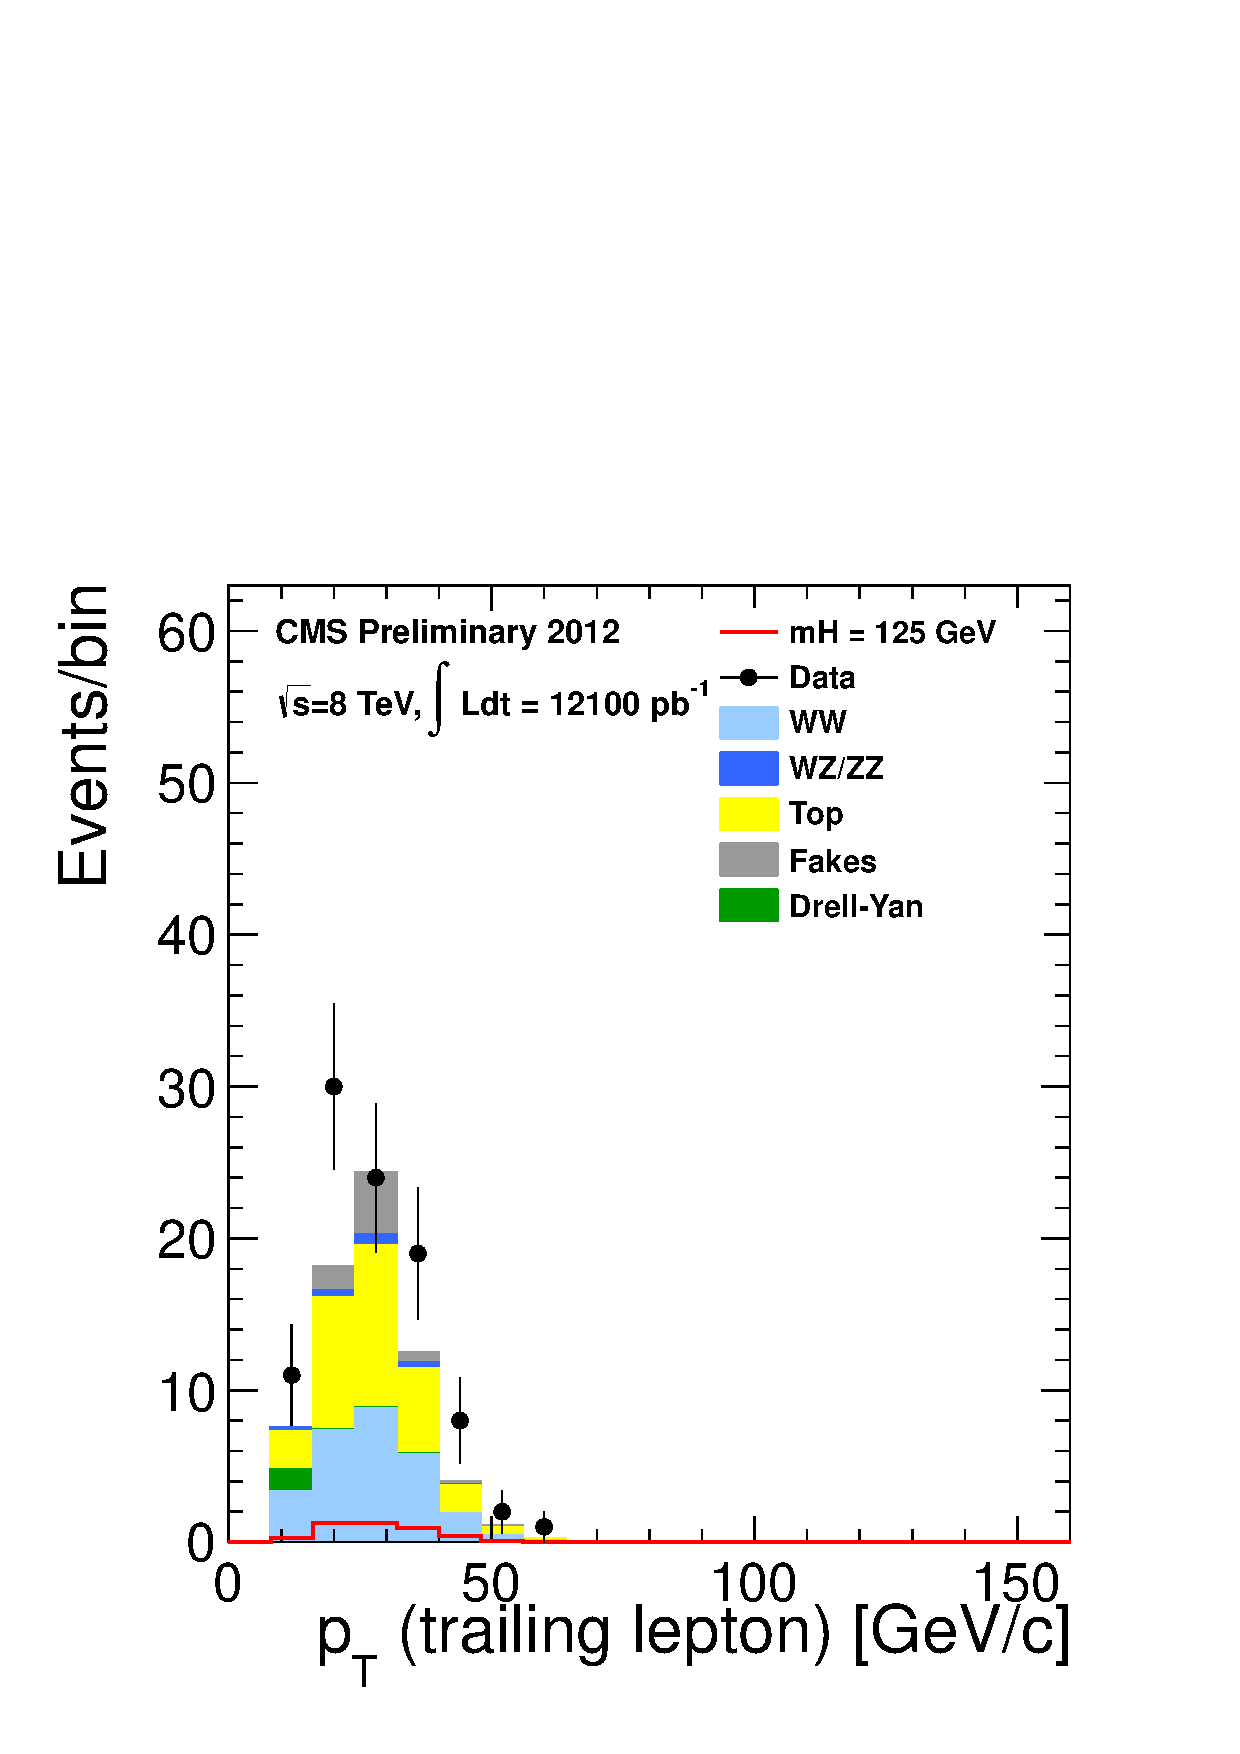
\includegraphics[width=.3\textwidth]{figures/hwwplots_mt120to140_mll25to50/hww_analysis18_125_ALL_of_1j_pt2.pdf}
}
\caption{The \ptlmin~distributions for $\mHi=125~\GeV$ with \intlumiEightTeV~of data in the 0-jet \subref{subfig:hww125_pt2_0j},
1-jet \subref{subfig:hww125_pt2_1j} bin analyses.}
\label{fig:hww125_pt2}
\end{figure} 


